% Ein Beispielkapitel
%

\chapter{Implementation}

The implementation which are done in this thesis aim at enabling the building and simulation
of a full mouse brain model relaying on point neuron model. Such a model must be build by
reconstructing parts of the model from experimental data provided by both the Allen Institute for
Brain for Science and the Blue Brain Project
To this aim, an efficient data format is defined, the circuit generation scripts are adapted to
run on a bigger scale and the NEST simulator is extended to load the new data format.

\section{Data formats}
A point neuron model contains point neurons and connections (synapses) between the point neurons.
The same point neuron model (conductance based exponential integrate-and-fire neuron model \cite{brette2005adaptive}) and synapse model (Tsodyks synapse model containing synaptic short-term depression and short-term facilitation \cite{tsodyks1997neural, fuhrmann2002coding}) are used for all neurons and synapses respectively.
The neurons and synapses are characterized by parameters.
Each neuron is defined by a given set of parameters.
The synapses contain besides the parameters the source and target neuron id, which the synapses connects.
To store the circuit in files two different data formats are defined.
The first data format defines the storage for all neuron parameters.
The second data format defines the storage for the synapse parameters and source and target neuron ids.

The data format for the neurons and the synapses follow two different concepts.
The neuron data format contains multiple datasets containing the neuron parameters.
All datasets have by definition the same length. This length defines the number of neurons.
The neuron parameters of neuron $i$ are stored in the i-th line of each data set.
Besides the neuron parameters the file contains attributes for storing meta data of the circuit.
\begin{figure}[ht!]
   	\begin{center}
        \subfigure[HDF5 file format for the neurons]{%
            \label{fig:allInjections}
            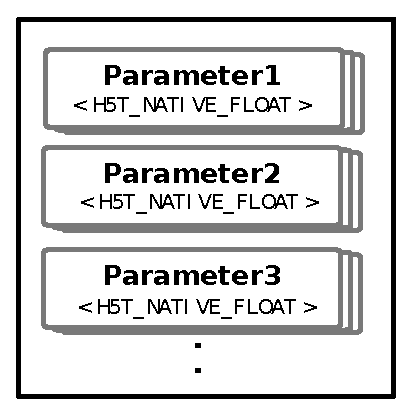
\includegraphics[scale=0.5]{pictures/hdf5_neuron_format.eps}
        }
        \hspace{1cm}
        \subfigure[HDF5 file format for the synapses]{%
            \label{fig:oneProjection}
            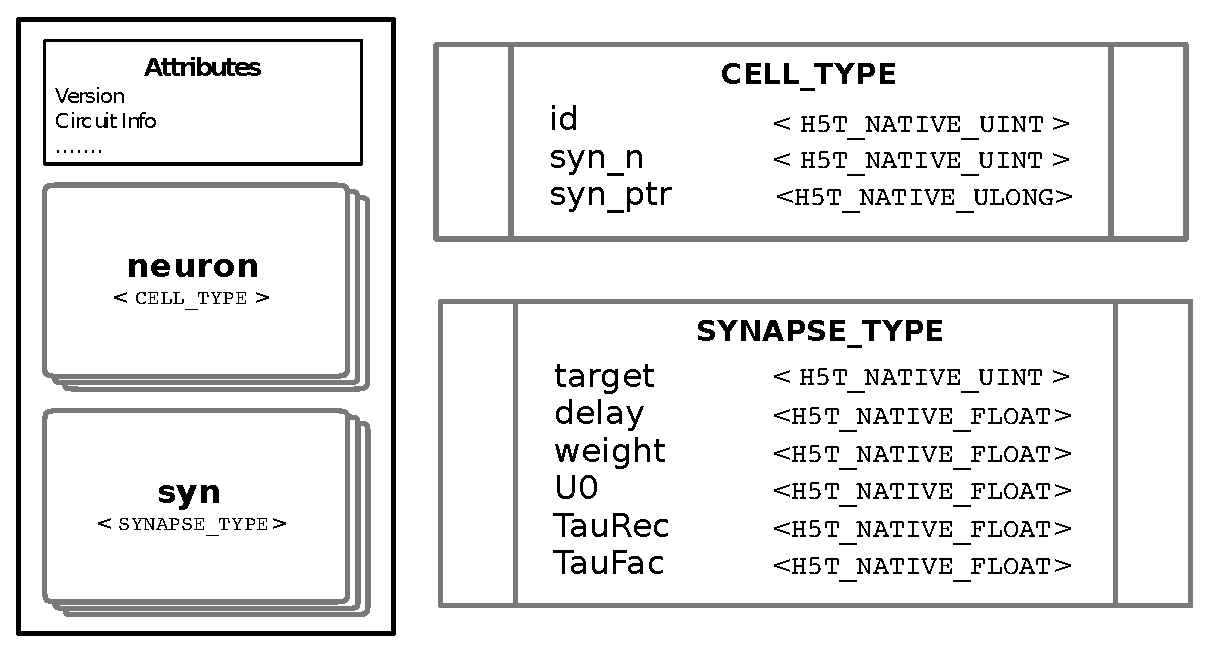
\includegraphics[scale=0.41]{pictures/hdf5_syn_format.eps}
       }
    	   \end{center}
    	\caption{%
        You can see the data format with their related datasets and data types. 
        How they are created by the circuit generation and loaded by the NEST import module.
     }%
   \label{fig:atlas}
   \end{figure}
The synapse data format contains only two datasets. In general the datasets contain for each synapse
a source neuron id, a target neuron id and a set of parameters. To reduce the amount of data.
The source neuron ids are grouped together in the \emph{neuron} dataset. This is feasible, because
the number of synapses is way bigger than the number of source neurons ($~11,000$ synapses per source neuron).
The \emph{syn\_ptr} value defines the related starting index in the \emph{syn} dataset,
respectively \emph{syn\_n} defines the number of related following entries.
The \emph{syn} dataset contains the target neuron id and a set of parameters.
Both datasets use a compound data type to store different data types in the same dataset.

\newpage
\section{Circuit generation}
Rewriting the sequential python script to a hybrid C++ application require a parallel implementation of the algorithm and the usage of 
a parallel random generator. For the parallelization strategy a Master-Slave approach is chosen to distribute the workload dynamically on the processes.
Communication between the individual processes is not necessary. Only the workload management is handled by the master process.
For the random generator Random123\cite{salmon2011parallel} is used.
It ensures reproducible results without correlations in the generated values, which is essential.


%%insert somewhere
%Unfortunately all injections from these experiments do not
%cover the whole brain. So there are neurons which are not injected
%by any experiment. Therefore all neurons which are not injected should use the projection
%from the nearest injection.


\subsection{Long range connections}

The long range generation algorithm is adapted to be parallelizable efficiently.
The problem with the sequential algorithm is, that it iterates through all experiments
and generates all connections for all the voxels inside its injection regions, if 
all experiments before have not touched the voxels or have higher total injection
value. This means it generates connections which might be overwritten and each iteration might depend
on all previous iterations. To overcome the dependency the best chosen injection per voxel is calculated before hand.
The number of written entries can be calculated before hand. This allows to create
the HDF5 dataset before and assign a writing position to each voxel.
Thus all processes can write independent to the file system.
After that all voxels are distributed to the processes and inside the iteration over all neurons
inside the given voxel, the sequential algorithm can be applied on each process.
An efficient parallel implementation depends on the distribution of the voxels, which are
work packages for each process. The work load has to be distributed equally on all processes.
Therefore the determination of the wall-clock time needed for each voxel is necessary.
But it \ref{eq:L} is not constant.
So the algorithm can be partitioned into five parts: linear rejection (\emph{linear}), storing to disk \emph{store}(),
loading experiment data (\emph{load}), select neurons in injection (\emph{selI}), select neurons in projection (\emph{selP}).
\begin{equation} \label{eq:L}
	L \approx L_{linear}(n,m,M) + L_{store}(n,\omega) + L_{load}(\nu) + L_{selI}(n) + L_{selP}(m,\nu)
\end{equation}
$L_{load}(\nu)$, $L_{selI}(n)$ and $L_{selP}(m,\nu)$ are neglectable.
$\Omega$ and $\frac{\partial L_{linear}(n,m,M)}{\partial M}$  can not be estimated satisfyingly.
$\Omega$ represents waiting times, which occur from independent parallel write operations.
$M$ represents the distribution of probability values.
The distribution effects the number rejections inside the linear rejection method.
Therefore it has a significant impact on the wall-clock time.
Thus there is only a rough estimation of the wall-clock time per voxel iteration possible.
\begin{equation} \label{eq:Lapprox}
	L_{estimate} = L_{linear}(n,m) + L_{store}(n)
\end{equation}
Therefore a statically and dynamically voxel distribution is implemented.
At first a third of all voxels are distributed (using algorithm \ref{alg:distributeWeightedVoxels}) based on the weight $L_{estimate}$ \ref{eq:Lapprox}  per voxel.
\begin{algorithm}[ht!]
\KwData{List of all voxels with weights}
\KwResult{List of private voxels and sum of weights per process}
\For{voxel n}{
	Find Process with smallest sum of weights \\
	Add weight to sum of weights of Process \\
	\If{Process is me}{
		Add voxel to private voxel list
	}
}
\caption{Algorithm to distribute weighted voxels to processes}
\label{alg:distributeWeightedVoxels}
\end{algorithm}
After that the master process distributes further voxels in sets on request from the other processes.
Figure \ref{fig:longrangParallel} illustrates the workflow of all processes.
\begin{figure}[ht!]
\centering
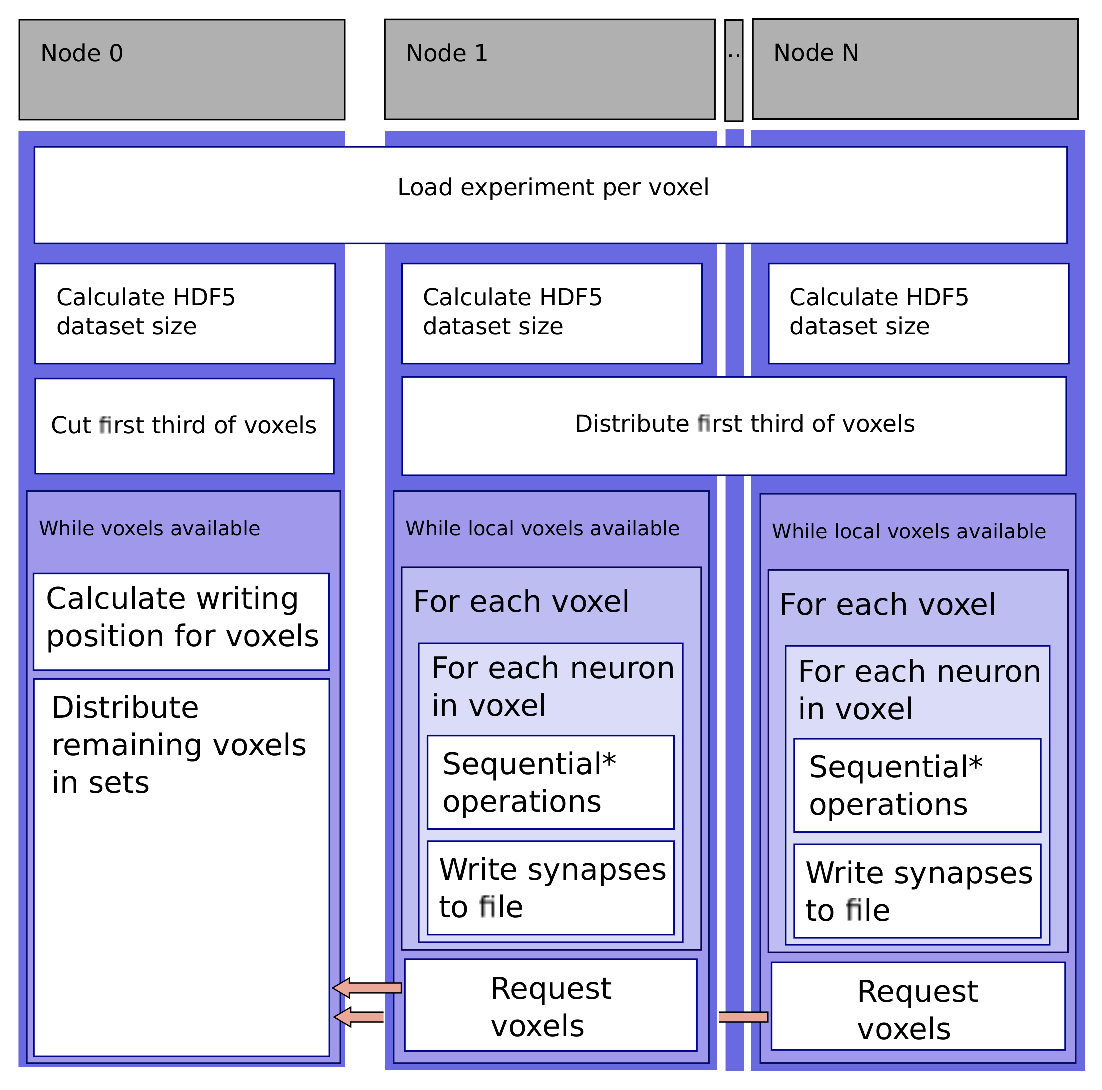
\includegraphics[scale=0.5]{pictures/longRange_parallelAlg.eps}
\caption{Task distribution between the processes for the long range connections generation. It illustrates which tasks are distributed between which processes.}
\label{fig:longrangParallel}
\end{figure}
\emph{Process 0} is selected as the master process. It does not participate on the iterations.
It manages the dynamic distribution of the voxels to the other processes and 
assigns write positions to each voxels. Thus each process receives besides the 
voxel information the positions,
where it has to write its data to the HDF5 datasets.
\begin{figure}[ht!]
\centering
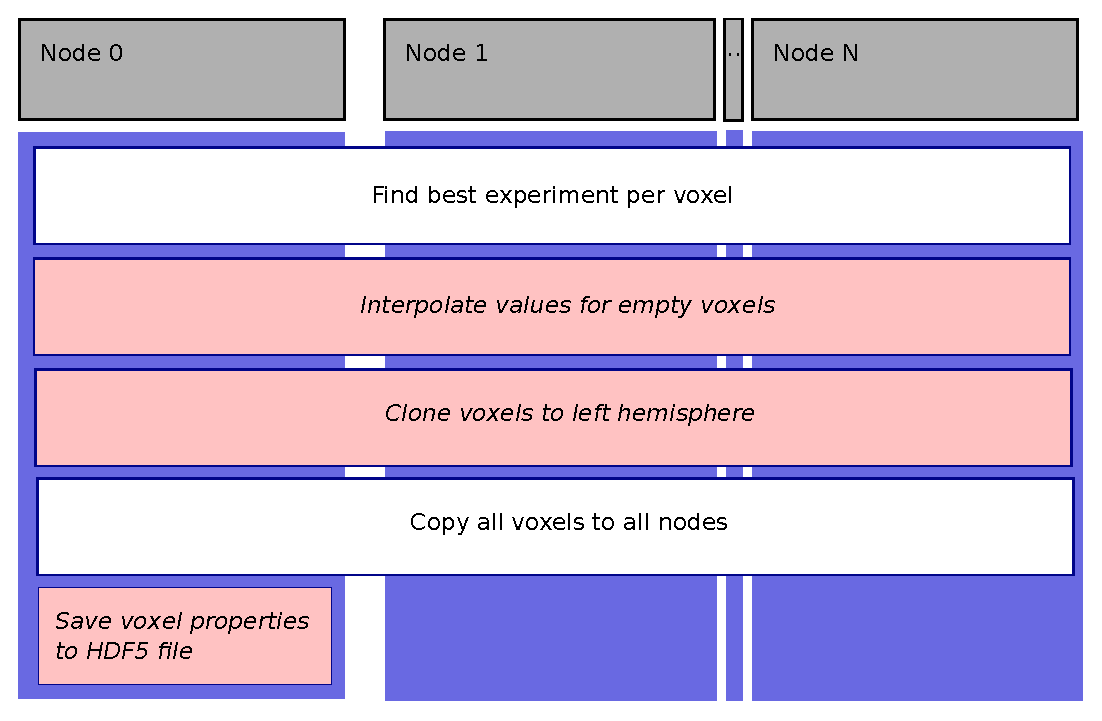
\includegraphics[scale=0.5]{pictures/longRange_BestExp_parallelAlg.eps}
\caption{Subtasks of the above listed \emph{Load experiment per voxel} task}
\label{fig:longrangeLEPV}
\end{figure}
Task \emph{Load experiment per voxel} from Figure \ref{fig:longrangParallel} contain several subtasks.
It generates the voxel datasets, which are distributed afterwards.
Manipulations of the generation effect mostly this part.
So the part allows modifications of the applied functionalities. 
Further the whole function can be skipped by loading the voxel information from file \ref{file:voxelinfo}.
Figure \ref{fig:longrangeLEPV} shows the subtasks.
The red tasks are optional and can be activated via command line arguments.
In the first task \emph{Find best experiment per voxel} each process loads a set of experiments.
Iteratively the experiment with the smallest total injection density is assigned to each voxel
on each process. Afterwards a MPI reduction function returns the smallest value for each voxel on
each process.
But there are regions which were not injected by any experiment available.
So there is no connection information available for the internal neurons.
To overcome the missing data a piecewise constant interpolation is applied to the chosen experiment per voxel
in \emph{Interpolate values for empty voxels}.
It is realised with an distributed iteratively nearest neighbour search algorithm for each missing voxel.
Figure \ref{longrange} shows an illustration of the search algorithm
projected in a 2D plane. 
\begin{figure}[ht!]
\centering
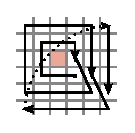
\includegraphics[scale=2.5]{pictures/longRange_Nearest_parallelAlg.eps}
\caption{Find nearest neighbour loop}
\label{longrange}
\end{figure}
The first voxel along the search direction which is found is declared as the nearest neighbour.
The chosen experiment from the nearest neighbour is adopted.

Afterwards the voxels are mirrored from the right to the left hemisphere, because the
Allen Brain Atlas mostly delivers injection sites for the right hemisphere and
the mouse brain model is assumed to be symmetric.

Finally all voxel information are gathered to all processes.
For debugging or manipulating purposes function \emph{Save voxel properties to HDF5 file} can be used
to save the generated voxel information to file (see chapter \ref{file:voxelinfo}).

%\begin{figure}[ht!]
%   	\begin{center}
%        \subfigure[All nodes are equal and process the work based on a static distribution]{%
%            \label{fig:shortColumn}
%            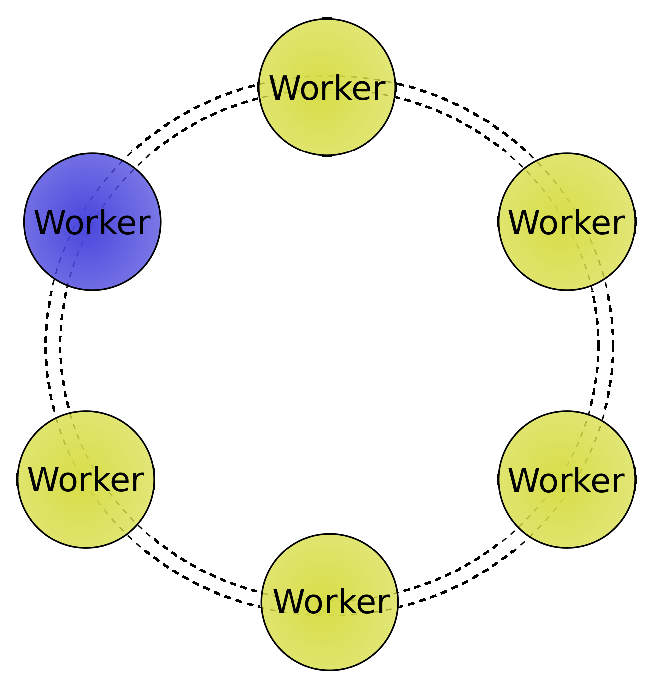
\includegraphics[scale=0.5]{pictures/All_Worker_Collective.eps}
%        }
%        \hspace{1cm}
%        \subfigure[The 0 node is assigned as the master node and handles from this on the management of the work distribution.]{%
%            \label{fig:shortColumnInCircuit}
%            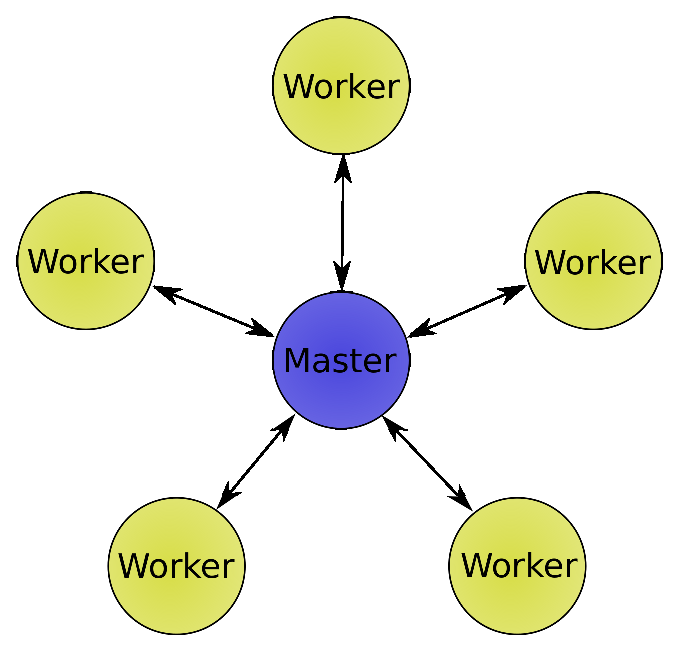
\includegraphics[scale=0.5]{pictures/MasterWorker.eps}
%       }
%    	   \end{center}
%    	\caption{%
%        The figure illustrates the work distribution and communication between the nodes.
%     }%
%   \label{fig:atlas}
%   \end{figure}


\subsection{Short range connections}

The algorithm \ref{alg:BBP} presented in the analysis section can be parallelized straight forward.
Each iteration is independent. The challenging part is the distribution of the iterations and
the writing to disk. The number of synapses which are created is not know. It is only available
at the end. Therefore all synpases are stored inside memory during the iterations and only written to disk 
at the end.

\begin{figure}[ht!]
\centering
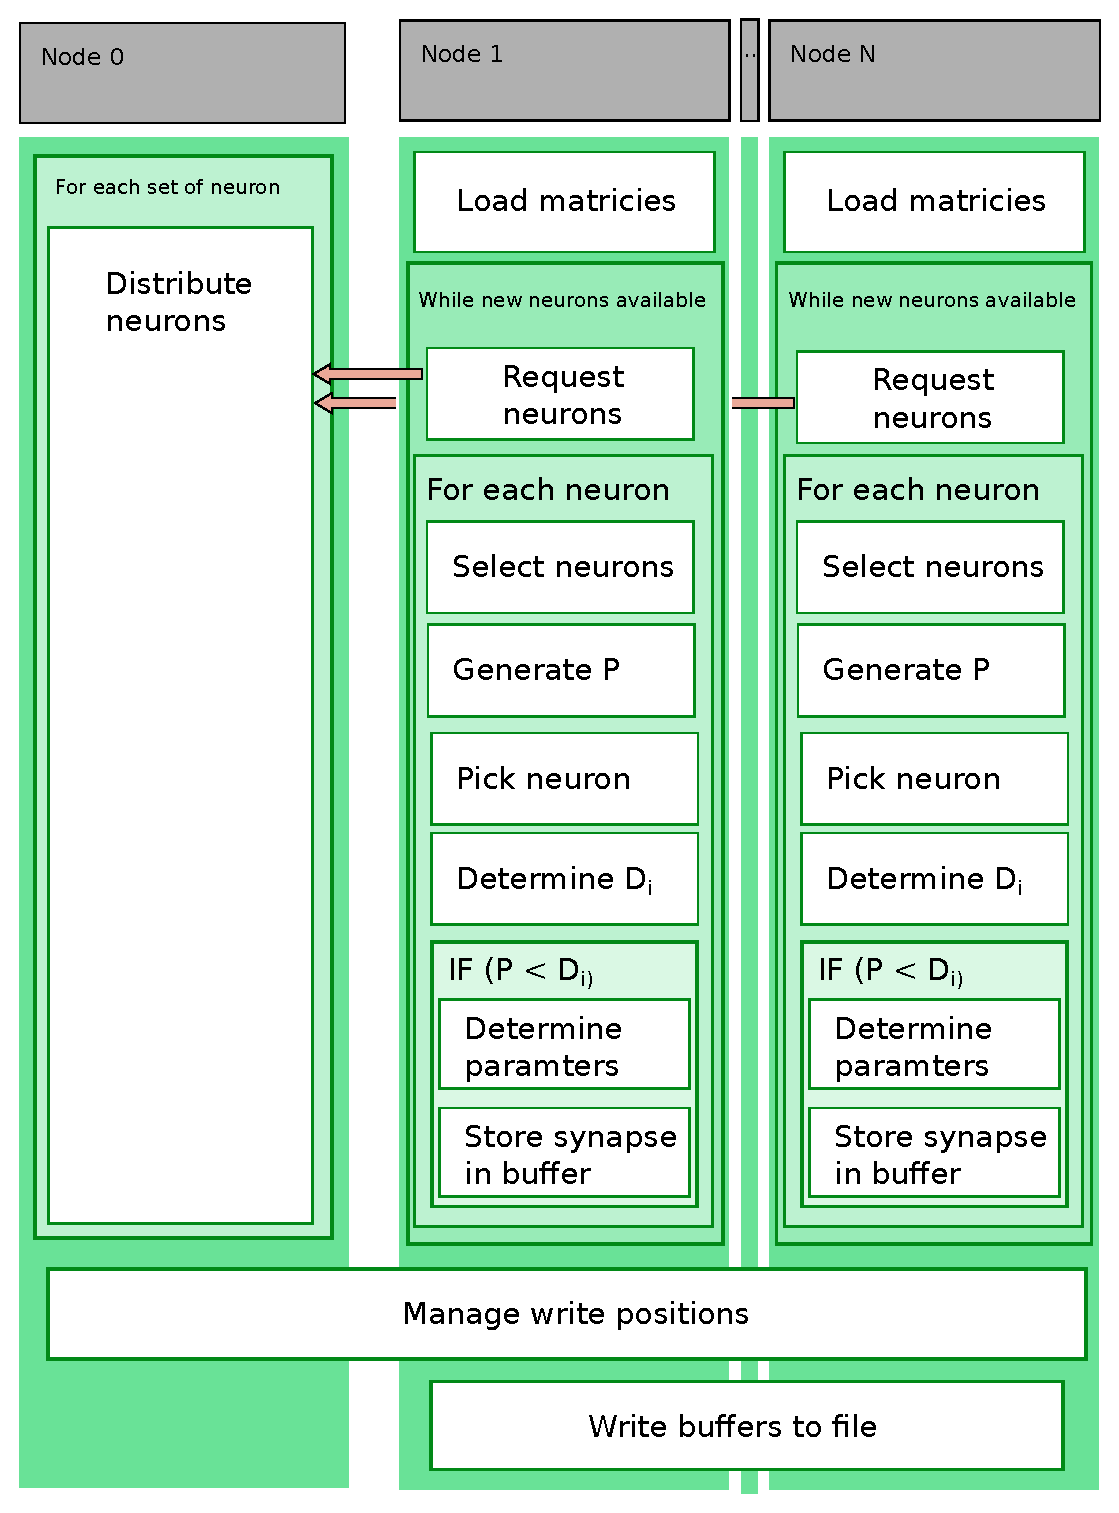
\includegraphics[scale=0.5]{pictures/shortRange_parallelAlg.eps}
\end{figure}

The iterations from the main loop from the sequential algorithm \ref{alg:BBP} are distributed between the processes.
The short range algorithm follows the same concepts as the long range generation parallelization.
The iterations are distributed first statically and afterwards dynamically.
The master process\emph{Process 0} handles the dynamic distribution management.
To overcome that the dynamical distribution becomes a bottleneck in the beginning a third of the iterations are distributed
statically between the working processes beforehand.
The work-load per neuron is not estimated in advance.
The iterations are partitioned continuously without weights.
Each process of the workes (all processes expect of \emph{Process 0}) receives the neurons with the ids $x_{process_id-1}$
to $x_{process_id}$ (\emph{Process 0} is not part of distribution. It is skipped.).
$x_i$ relates to equation \ref{eq:process2id}.
\begin{equation}
	x_i = round(i * \frac{N_{neurons}}{N_{processes}-1})
	\label{eq:process2id}
\end{equation}
During runtime the master process manages the distribution of the neurons. For each neuron 
its synapses have to be created. The workers load in the first step all needed matrices from the file system.
Then each process request a set of neurons from the master process. Over this set it iterates and creates resulting
synapses. The library Random123 is used to get values for the random variable. Therefore a parallel usage of 
the given sequential algorithm is possible. Only the storage of the generated synapse list, has to be done 
after all iterations. So in each loop the synapse list is stored in a buffer.
The buffer is based on an own implemented queue class. It nests standard vectors.
It contains one vector of fixed size vectors, which contain the synapse objects.
It allows to increase the buffer size efficiently. The buffer size is adapted to 
the memory available on the used Blue Gene Q systems.
Also the buffer can be written to disk efficiently, because the sub vectors are
accessible and can be written as chunks to file.
If all neurons are distributed and processed, all processes, including the master process, calculate the writing position
in the HDF5 datasets where each process has to write its data to. After that all workers write theirs synapse lists to
disk.


%\begin{figure}[ht!]
%   	\begin{center}
%        \subfigure[Master-worker strategy to get good balance properties]{%
%            \label{fig:shortColumn}
%            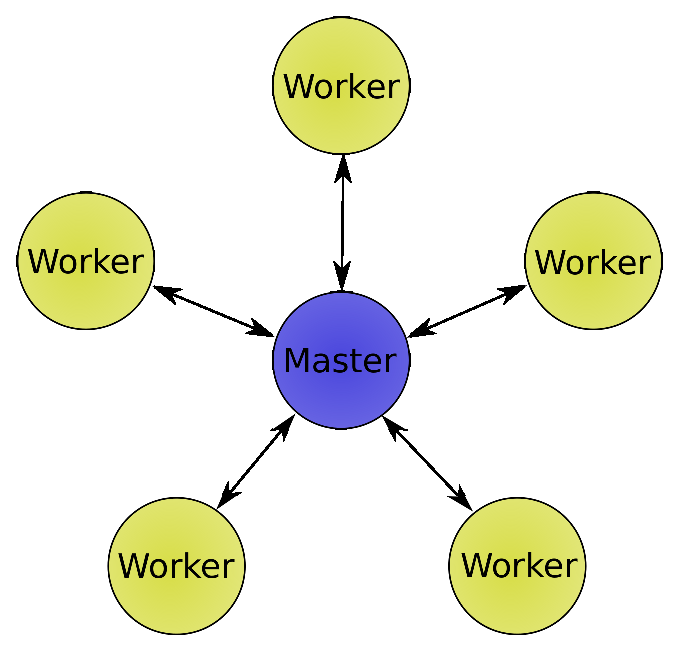
\includegraphics[scale=0.5]{pictures/MasterWorker.eps}
%        }
%        \hspace{1cm}
%        \subfigure[Collective write operation to maximize used bandwidth]{%
%            \label{fig:shortColumnInCircuit}
%            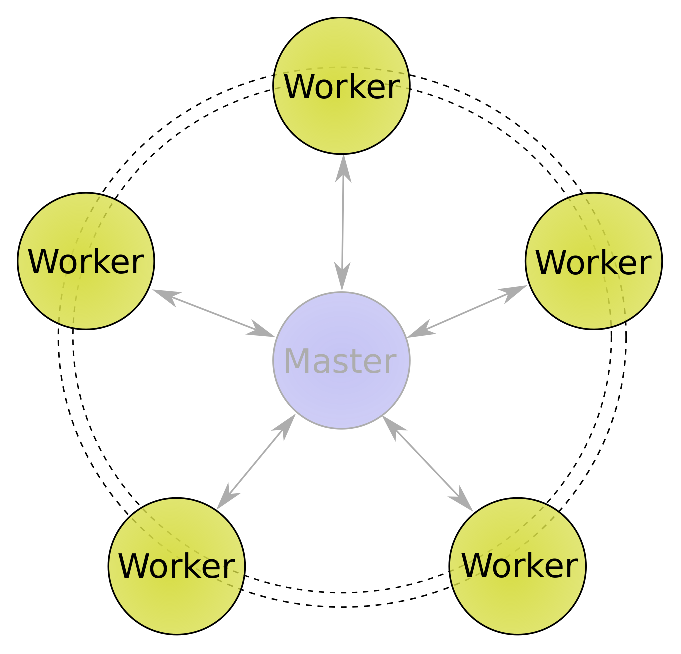
\includegraphics[scale=0.5]{pictures/Worker_Collective.eps}
%       }
%    	   \end{center}
%    	\caption{%
%        The figure illustrates the work distribution and communication between the nodes.
%     }%
%   \label{fig:atlas}
%   \end{figure}


\newpage
\section{Circuit validation}
In the context of this thesis the circuit is validated in terms of geometrical correct placement of
the synapses. So the position of the source and target can be visualized and be compared to a 
reference system. For the long and the short range connectivity the geometrical shape is know.
In particular the long range connectivity should connect neurons from the injected regions to neurons
in the projected region for each used experiment. Therefore a circuit for a single experiment is 
generated, the target and source neurons are visualized in a 3D coordinate system and the the injection
and projection is used as the reference system. If source neurons are inside the injection space and all
target neurons are in the projection space, the implementation is correct.
For the short range connectivity all post-synaptic neurons of synapses having the same pre-synaptic neuron should
lay inside a cylinder in layer 1 to 6. Visualising the post-synaptic neurons geometrical on top of the contour of layer 1 to 6 allows to review if the shape matches with a cylinder.
To perform the visual validation the renderer voxalize \ref{voxelize} is used with the visualization tool Paraview \ref{paraview}.
 \begin{figure}[ht!]
\centering
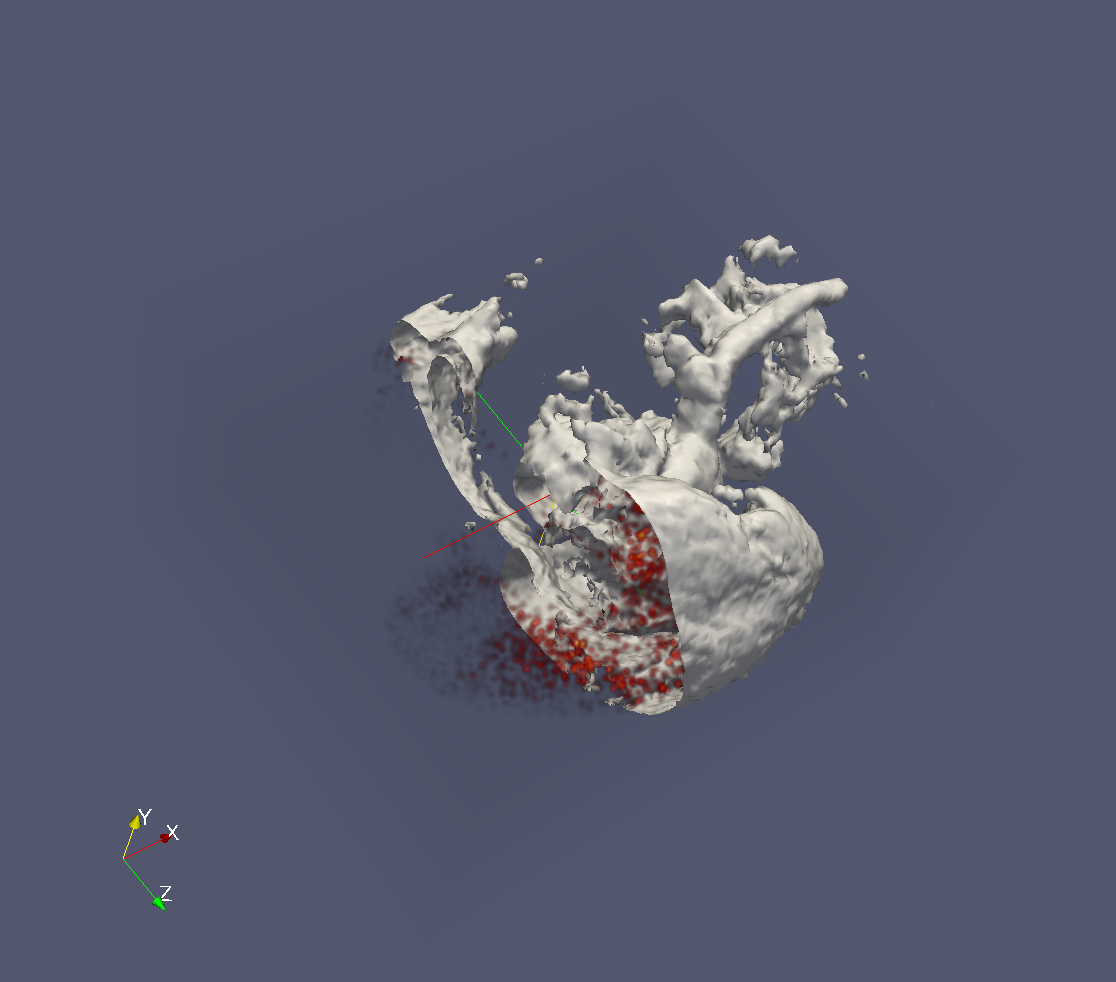
\includegraphics[width=0.4\textwidth]{pictures/paraview_ex.png}
\end{figure}
For the validation the BBP visualization team offered a rendering pipeline to visualize the placement of target neurons for each synapse file. Therefore the neuron and synapse HDF5 can be imported into 
Voxelize \ref{voxelize}. Voxelize creates a voxelized dataset out of the target neuron positions, which can be exported into
a MetaImage \ref{MetaImage} file or directly viewed with Livre \ref{Livre}.
The MetaImage files can be viewed with Paraview \ref{Paraview}.
Injection and projection images are also given in the MetaImage format.
A direct comparison inside of Paraview is possible.
Loading the projection inside of Paraview and applying the contour filter on it with a threshold of $0.01$ (threshold is also applied to the same data in the long range connectivity generation) allows to visualize the valid boundaries for all target neurons for this particular experiment.
 
\begin{itemize}
      \item Pictures of both validation
      \item Visual validation of spiking activity
      \item Statistical properties are not analyzed in this work 
\end{itemize}

\section{NEST import modules}
The neuronal spiking network simulator NEST is developed in \emph{C++} and delivers
an user interface based on an own description language \emph{SLI} and  and a Python interface.
The new use case shall be integrated into the standard work flow of NEST.
To this end, the functionality in \emph{C++} the interfaces have to be extended.
The difficulties of the network generation is based on a difference in 
the NEST internal data structure and the data delivered by the Allen Institute.
Connection information contains target and source neurons besides biochemical
information of the synapses. Because of the in vitro injection methods the
connection information maps the synapse from the source to the target neurons.
For multi process simulations NEST distributes all neurons based on a modulo function 
to the processes. Because of memory optimizations the synapses are only stored on the
post synaptic process. This means that the connection information is stored
on the process, where the target neuron is located. Therefore a transformation of the given data is
necessary. Preprocessing of the input data should be avoided as far as possible to capture
future use cases.
The resulting implementation shall load the connection information efficiently in parallel,
distribute the synapse information to the post synaptic process and store it in
the NEST data structure.
Further requirements of the implementation are an efficient use of the available resources as
memory and computation power. 


\lstdefinestyle{cppcode} {language=C++,
                basicstyle=\small\ttfamily,
                keywordstyle=\color{blue}\ttfamily,
                stringstyle=\color{red}\ttfamily,
                commentstyle=\color{green}\ttfamily,
                morecomment=[l][\color{magenta}]{\#}
                numbers=left,
  				stepnumber=5,    
  				firstnumber=1,
 				numberfirstline=true
}

\subsubsection{Import neurons}
The internal c++ API of NEST allows creation and manipulation of the circuit.
The API is mainly developed to be an interface between the internal structure
and the SLI interface. But my implementation accesses the c++ functions directly,
to avoid the SLI layer. To access the API in between the internal NEST classes
have to be analysed. Because I am facing the execution on large scale machines,
I focus on thread-safty and locality of internal circuit generation functions.
Which means, I focus on how NEST internally distribute the data and on which processes, which
function have to be called.

NEST does not support information exchange during the internal circuit generation. 
To create neurons inside the circuit the equal function call has to be
performed on all processes. NEST itself sorts out, which information is needed on which process.
But by analysing the NEST code I found out that not all function calls are necessary on all processes.
The creation of objects (\ref{code:addnode}) has to performed on all processes.
\begin{figure}[ht!]
\begin{lstlisting}[style=cppcode]
/*** Add a number of nodes to the network.
   * This function creates n Node objects of Model m and adds them
   * to the Network at the current position.
   * @param m valid Model ID.
   * @param n Number of Nodes to be created. Defaults to 1 if not
   * specified.*/
  index add_node( index m, long_t n = 1 );
\end{lstlisting}
\caption{NEST internal add\_{}node function to create neurons and subnets.}
\label{code:addnode}
\end{figure}
Thus the number of subnets and neurons have to be known on all processes.
The neurons are created inside of the current subnet.
By default this is the root node of NEST.
The current subnet can be changed by calling the function beforehand.
\begin{figure}[ht!]
\begin{lstlisting}[style=cppcode]
/** Change current working node. The specified node must
   * exist and be a subnet. */
  void go_to( index );
\end{lstlisting}
\caption{NEST internal go\_{}to function to change the subnet.}
\label{code:addnode}
\end{figure}
But the assignment(\ref{code:setstatus}) of model parameters can be performed only on the processes,
where the object is stored.
\begin{figure}[ht!]
\begin{lstlisting}[style=cppcode]
/*** Set properties of a Node. The specified node must exist. */
  void set_status( index, const DictionaryDatum& );
\end{lstlisting}
\caption{NEST internal set\_{}status function to set model parameters of neurons.}
\label{code:setstatus}
\end{figure}
This allows to only load and assign the parameters on the corresponding process.
Therefore knowing the distribution of neurons on the processes is essential.
It is based on the modulus function \ref{NEST}.
Process with id $i$ is stored on process $i mod N_{processes}$.

To group neurons together to subnets, neurons can be created inside of virtual subnets.
This subnets have to be created before hand.
Therefore the implemented algorithm sorts out the needed subnets in its first step.
\begin{algorithm}
 \KwData{HDF5 neuron dataset}
 \KwResult{Created neurons inside NEST data structure}
 Find unique values in subnet dataset; \\
 Create subnet for each unique entry; \\
 Create neurons based on length of HDF5 datasets with given neuron type inside specified subnets; \\
 Read parameter datasets collectively; \\
 Assign parameters to neurons;
\label{alg2}
\caption{Implemented import neurons algorithm}
\end{algorithm}
Unique values are extracted from the subnet dataset.
After that for each unique value a subnet is created.
In the next step the neurons are iteratively created inside the specified subnet.
Then needed parameter values are loaded from the HDF5 datasets and assigned to the neurons.
Derived from the distribution function (see \ref{}) each process has to load $N_{processes}$
entries starting from its process id.

\newpage
\subsubsection{Import synapses}
The synapse import module is based on the same concept as the import neuron module.
The synapse creation functionality of NEST is analysed.
Needed functions are reviewed for thread-safeness and locality.

Further an algorithm is implemented which arranges the given data on disk into
the needed structure.

To store a given synapse into the NEST data structure,
the \emph{connect} function \ref{code:connect} is used.
It supports the passing of synapse parameters and is thread-safe.
\begin{figure}[ht!]
\begin{lstlisting}[style=cppcode]
/*** Connect two nodes. The source node is defined by its global ID.
   * The target node is defined by the node. The connection is
   * established on the thread/process that owns the target node.
   *
   * The parameters delay and weight have the default value NAN.
   * NAN is a special value in cmath, which describes double values that
   * are not a number. If delay or weight is omitted in an connect call,
   * NAN indicates this and weight/delay are set only, if they are valid.
   *
   * \param s GID of the sending Node.
   * \param target Pointer to target Node.
   * \param target_thread Thread that hosts the target node.
   * \param syn The synapse model to use.
   * \param params parameter dict to configure the synapse
   * \param d Delay of the connection (in ms).
   * \param w Weight of the connection. */
  void connect( index s,
    Node* target,
    thread target_thread,
    index syn,
    DictionaryDatum& params,
    double_t d = NAN,
    double_t w = NAN );
\end{lstlisting}
\caption{NEST internal connect function to create a synapse.}
\label{code:connect}
\end{figure}
It has to be called on the node where the post-synaptic neuron is located.
The synapses are grouped by pre-synaptic neurons.
Therefore the synapses have to be rearranged before they can be connected efficiently.

The developed algorithm \ref{alg2} loads the synapses from file, rearranges the order
among nodes and calls the connect function for each synapse on the correct process.
\begin{algorithm}
	\KwData{List of HDF5 files for each process, block size}
	\KwResult{Connected NEST network}
	\While{Block to read in HDF5 files}{
		Read block and store in memory \hspace{45px}(1)\;
 Determine target process for each synapse \hspace{63px}(1,2) \hspace{36px}$\mathcal{O}(n)$\;
 Sort synapses by target processes \hspace{66px}(1,2) \hspace{28px}$\mathcal{O}(n^2)$\;
 MPI\_Alltoallv using sorted list \hspace{76px}(1,2,3,4)\;
 Connect all synapses using NEST function \hspace{36px}(1,2) \hspace{45px}$\mathcal{O}(n)$\;
	}
	\caption{Implemented import synapses algorithm, $S_i$ source neuron $i$, $Tn_i$ target neuron $i$.
	set in brackets contains current needed variables}
\label{alg2}
\end{algorithm}

At first the each node loads the pre-synaptic neuron ids from \emph{neuron} dataset to memory.
After that each iteration reads block-wise a set of synapses from \emph{syn} dataset and
stores them inside a vector of synapse objects.
Then the pre-synaptic neuron ids are integrated into each synapse object.
Each process contains a set of synapses now.
But most of synapses have to be transferred to different nodes.
Therefore the process (target process) where the post-synaptic neuron is located is determined (using equation \ref{eq:processfromid}).
To transfer it to the target process, all synapse vectors have to be sorted by the target vector.
After that \emph{MPI\_Alltoallv} is used to send the synapses from all to all processes.
Afterwards each process receives its list of synapses and can use the \emph{NEST} connect function, to copy it to its internal data structure.
The last step of the algorithm is 

Further the function call set\_{}status is thread-safe, because each
thread stores its neuron parameters in an own object.
But creating a \emph{DictionaryDatum} object is not thread-safe.
The emph{DictionaryDatum} object is necessary to pass the model
parameters to the neuron nodes. The creation and destruction of this
object refers to a memory stack object for SLI objects, which is an static object,
without thread-safety precautions. 


\begin{figure}[ht!]
\centering
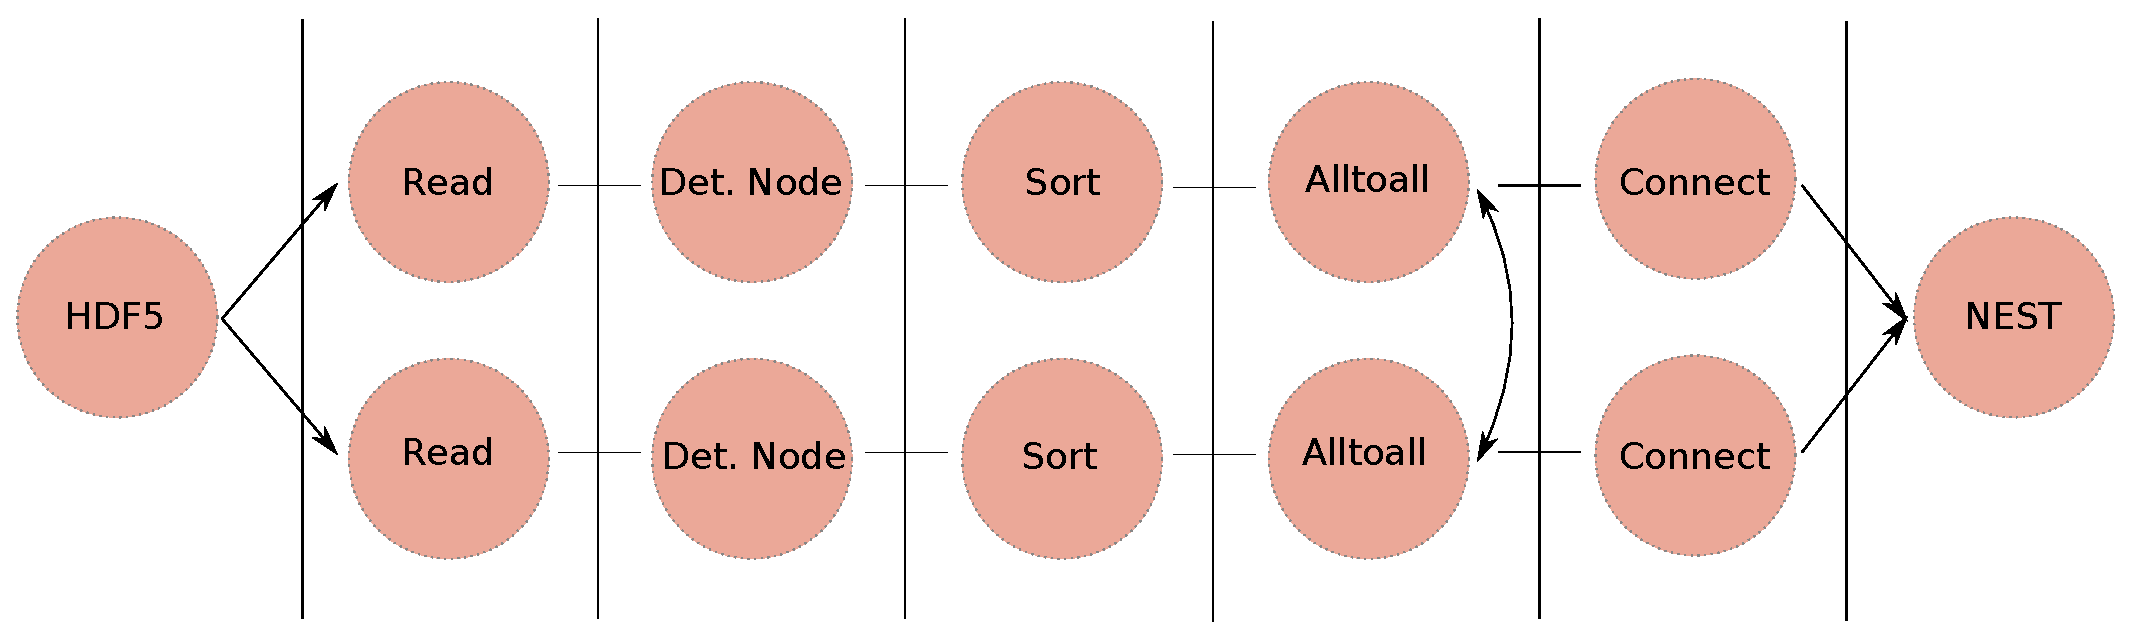
\includegraphics[scale=0.4]{pictures/Connect_inside_iteration.eps}
\caption{Inside iteration parallel workflow}
\label{Algparts}
\end{figure}

\begin{figure}[ht!]
\centering
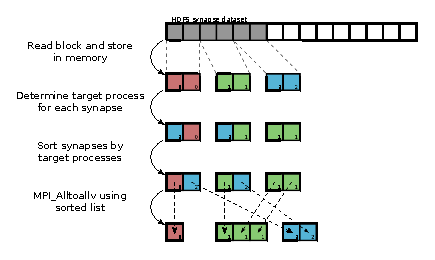
\includegraphics[scale=2.0]{pictures/import_syn_vis.eps}
\caption{Distribute synapses to processes.}
\end{figure}

\begin{figure}[ht!]
\centering

\includegraphics[scale=2.0]{pictures/import_syn_vis_second_it.eps}
\caption{Distribute synapses to processes.}
\end{figure}

\begin{figure}[ht!]
\begin{lstlisting}[style=cppcode]
void H5Synapses::singleConnect(NESTNodeSynapse& syn, 
    		index synmodel_id,
    		Node* const node,
    		const nest::thread thread,
    		DictionaryDatum& d, 
    		std::vector<const Token*> v_ptr)
{
  index source = synapse.source_neuron_;
  if (NestModule::get_network().is_local_node(target_node)) { 
    for (int i=2; i<prop_names.size(); i++) {
      double value = syn.prop_values_[i] * facts[i] + offsets[i];
      setValue<double_t>( *v_ptr[i], value );
    }
    NestModule::get_network().connect(source, node, thread,
                                      synmodel_id, d,
                                      syn.weight,
                                      syn.delay);
  }
  else {
    throw nest::IllegalConnection(..);
  }
}
\end{lstlisting}
\caption{}
\end{figure}

\newpage
\section{Memory consumption}
\begin{figure}[ht!]
\begin{tabular}{| l | l | l | l |}
    \hline
    (id) & data structures & memory consumption \\ \hline
    (1) & block in memory & $sizeof(float)*h*p$ \\ \hline
    (2) & target neuron node list & $sizeof(int)*h$ \\ \hline
    (3) & MPI send vectors & $(sizeof(float)*p + sizeof(int)) * h$ \\ \hline
    (4) & MPI recv vectors & $(sizeof(float)*p + sizeof(int)) * \frac{h}{\nu(N)}$ \\ \hline
    \end{tabular}
\caption{$N$: number of processes; $h$: size of block; $p$: number of parameters; $\nu(N)$: distribution coefficient of data}
\end{figure}
The maximum memory consumption is:
\begin{equation}
  M = (sizeof(float)*p + sizeof(int)) * 2h * (1 + \frac{1}{\nu(N)})
  \label{eq:maxmemoryconsumption}
\end{equation}
The block size $p$ is set to $1e6$ for the run on the BG/Q.
It affects the memory consumption and performance loading data from disk.
The implementation could handle different values per process.
But a block size adoption based on memory bottlenecks, is not implemented (see discussion \ref{pAdaption}).